%=====================================================
%====== If you are new to LaTeX, this website ========
%======     will be your new best friend:     ========
%======   http://en.wikibooks.org/wiki/LaTeX  ========
%======   Template created by Jonathan Blair  ========
%=====================================================



%=====================================================
%============ Controls ===============================
%=====================================================

%\documentclass[12pt,letterpaper,onecolumn]{article}
\documentclass[11pt,letterpaper,onecolumn]{article}
%\documentclass[10pt,letterpaper,onecolumn]{article}  % not recommended
%\documentclass[12pt,letterpaper,twocolumn]{article}
%\documentclass[11pt,letterpaper,twocolumn]{article}
%\documentclass[10pt,letterpaper,twocolumn]{article}


\usepackage{amsmath}
\usepackage{graphicx}
\usepackage{url}
\usepackage{textgreek}
\usepackage{float}
\usepackage{booktabs}
%\graphicspath{{path-to-folder-containing-necessary-graphics}{other folder as necessary}}


%=====================================================
%============ \begin{document} =======================
%=====================================================

\begin{document}

%=====================================================
%============ Title ==================================
%=====================================================

\title{\bf Observation of the Behavior of a Common Emitter Amplifier}
%\title{\Large\bf Larger, Bolded Title}

%=====================================================
%============ Author =================================
%=====================================================
\author{
 Jairo Portillo \\*
  \\*
 PHY 338K Electronic Techniques \\*
 Department of Physics \\*
 The University of Texas at Austin \\*
 Austin, TX 78712, USA
}
\date{March 10, 2016}

%\address{The University of Texas, Austin, Texas, 78712}

\maketitle

%=====================================================
%============ Abstract ===============================
%=====================================================

\begin{abstract}

In this lab, we will explore the behavior of a common emitter amplifier. We will observe how frequency can influence the gain of the Amplifier. We will estimate the input and output impedance of the emitter amplifier and the relationship frequency has with the gain and phase.   

\end{abstract}

%=====================================================
%============ Body of the article ==========================
%=====================================================

%=====================================================
%============ Section ==================================
%=====================================================

\section{Preperation}

In order to prepare for this lab, we must review the behavior of transistors and the behavior of the common emitter amplifier.

\begin{figure}[H]
    \centering
    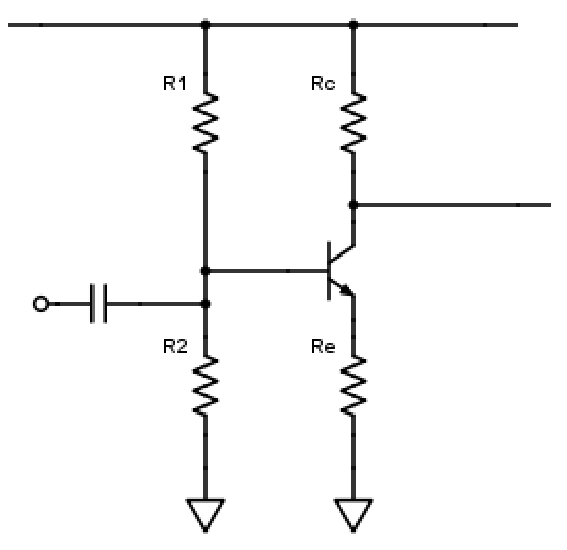
\includegraphics{circuit.pdf}
    \caption{Our common emitter amplifier circuit. With node as the AC input and a DC voltage input}
    \label{fig:my_label}
\end{figure} 
In Figure 1 we have our common emitter amplifier with a bypassed emitter resistor and a voltage divider. We already know that beta is 
$$\beta=\frac{I_C}{I_B}$$
where $I_C$ is the collector current and $I_B$ is the base current. The collector voltage can be found
$$V_{C}=V_{CC}-I_CR_C$$
where $V_{CC}$ is the DC input voltage that is used to amplify the signal and $R_C$ is the collector resistor. The capacitor so that a high pass filter can be formed with the voltage divider. 
$$C\ge\frac{1}{2\pi f(R_1\parallel R_2)}$$
where C is the capacitor, f is the frequency in Hertz, and $(R_1\parallel R_2)$ is the parallel resistance on the voltage divider $\frac{R_1 R_2}{R_1+R_2}$. The gain can be found with $gain = -\frac{R_C}{R_E}$.


\section{Lab work}

\subsection{Apparatus}

This lab will use a signal generator, an oscilloscope, a DC voltage source, a npn transistor, a .48 $\mu$F capacitor a 1 k$\Omega$, 10 k$\Omega$, and 100 k$\Omega$ variable resistors long with a 10 k$\Omega$ resistor. The AC signal generator will be in series with the 10 k$\Omega$ resistor and the base of the transistor. A Tee connector will connect the input AC signal with channel 1 on the oscilloscope. The emitter will be grounded and the collector will be connected to the 1 k$\Omega$ variable resistor, channel 2, and the DC voltage source. The DC voltage source will also behave as our ground. A representation of our circuit can be seen in Figure 1.  



\subsection{Data Collection}

In order to check the current gain $\beta$, we used the digital multimeter. For out npn transistor we found $\beta$ to be 186. Using the variable resistors, we set our resistances as the following: $R_1$ was at 82.4 k$\Omega$, $R_2$ was at 9.74 k$\Omega$, $R_C$ was at 7.86 k$\Omega$, and $R_E$ at .98 k$\Omega$. We kept $V_{CC}$ at 15 V DC and our input and 2.6 V AC sine wave. With these specification we was that amplification occurred between 80 Hz to 100 kHz where it would range from 2.6 V to 13.8 V before decreasing again. 

The Q point can be found with $\frac{V_{CC}}{2}$ and $\frac{I_C}{2}$. Using 
$$I_C = \frac{V_B}{R_E} \text{ and } V_B=\frac{R_2}{R_1 + R_2}V_{CC}$$
thus we see that 
$$I_C = \frac{R_2}{R_2+R_1}\frac{V_{CC}}{R_E}$$

Therefore we get a Q point at 7.5 V and 1.62 mA. We find our input impedance to be $Z_{in} = \beta R_E$ which turns out to be 182.28 k$\Omega$. Then if we solve for gain using $\frac{R_C}{R_E}$, we find 8.02 which gives us an output impedance of 22.7 k$\Omega$.
We can see the cut off frequency by solving for frequency from
$$C\ge\frac{R_1R_2}{2\pi f(R_1+R_2)}$$
and we see the frequency becomes 
$$f\ge\frac{R_1R_2}{2\pi C(R_1+R_2)}$$
and we find thet $f\ge 2GHz$. However if we replace $(R_1\parallel R_2)$ with the input impedance of 182.28 k$\Omega$ we find that $f\ge1.81Hz$ thus our cut off frequency is about 2 Hz which follow our observations of amplification at 80 Hz.
Using 
$$f\ge\frac{1}{2\pi CZ_{in}}$$
and solving for $Z_{in}\ge \frac{1}{2\pi Cf}$ we find that the dependence of gain on frequency is 
$$ Gain \approx Z_{out}2\pi Cf$$
\section{Summary and conclusions}

In this lab, we have seen how a common emitter amplifier can influence a signal based on the frequency. We found an input impedance of 182.28 k$\Omega$ and an output impedance of 22.7k$\Omega$. We find that the gain is 8.02 and is dependent on frequency with $ Gain \approx Z_{out}2\pi Cf$. Our amplifier has a cut off frequency of bout 2 Hz and would amplify the signal from 80 hZ to 100 kHz.



%=====================================================
%============ Bibliography  ==============================
%=====================================================



%=====================================================
%============ End ====================================
%=====================================================

\end{document}

%=====================================================
%============ End ====================================
%=====================================================